\documentclass[12pt]{article}
\usepackage[utf8]{inputenc}
\usepackage{geometry}
\usepackage{pdfpages}  % 导入pdfpages宏包
\geometry{a4paper, margin=1in}
\usepackage{fbox}

\begin{document}


\begin{flushright}
    \Large{\textbf{ISYS2120 Sem2, 2024}}
\end{flushright}

\begin{center}
    \LARGE{\textbf{Assignment 2 Group Report}} \\
    \vspace{2cm}
    
    \setlength\fboxsep{10pt}
    \setlength\fboxrule{1pt}
    \fbox{
        \parbox[c][3cm][c]{10cm}{
            \centering Group code: \\
            \vspace{0.5cm}
            \texttt{Asst2\_Lab18\_5B}
        }
    }
    
    \vspace{2cm}
    
    \fbox{
        \parbox[c][3cm][c]{10cm}{
            \centering Group members: \\
            \vspace{0.5cm}
            \texttt{Yicheng Shan \\Mingyuan Ba}
        }
    }
    
    \vspace{2cm}

\end{center}

\newpage

\section*{Part A}
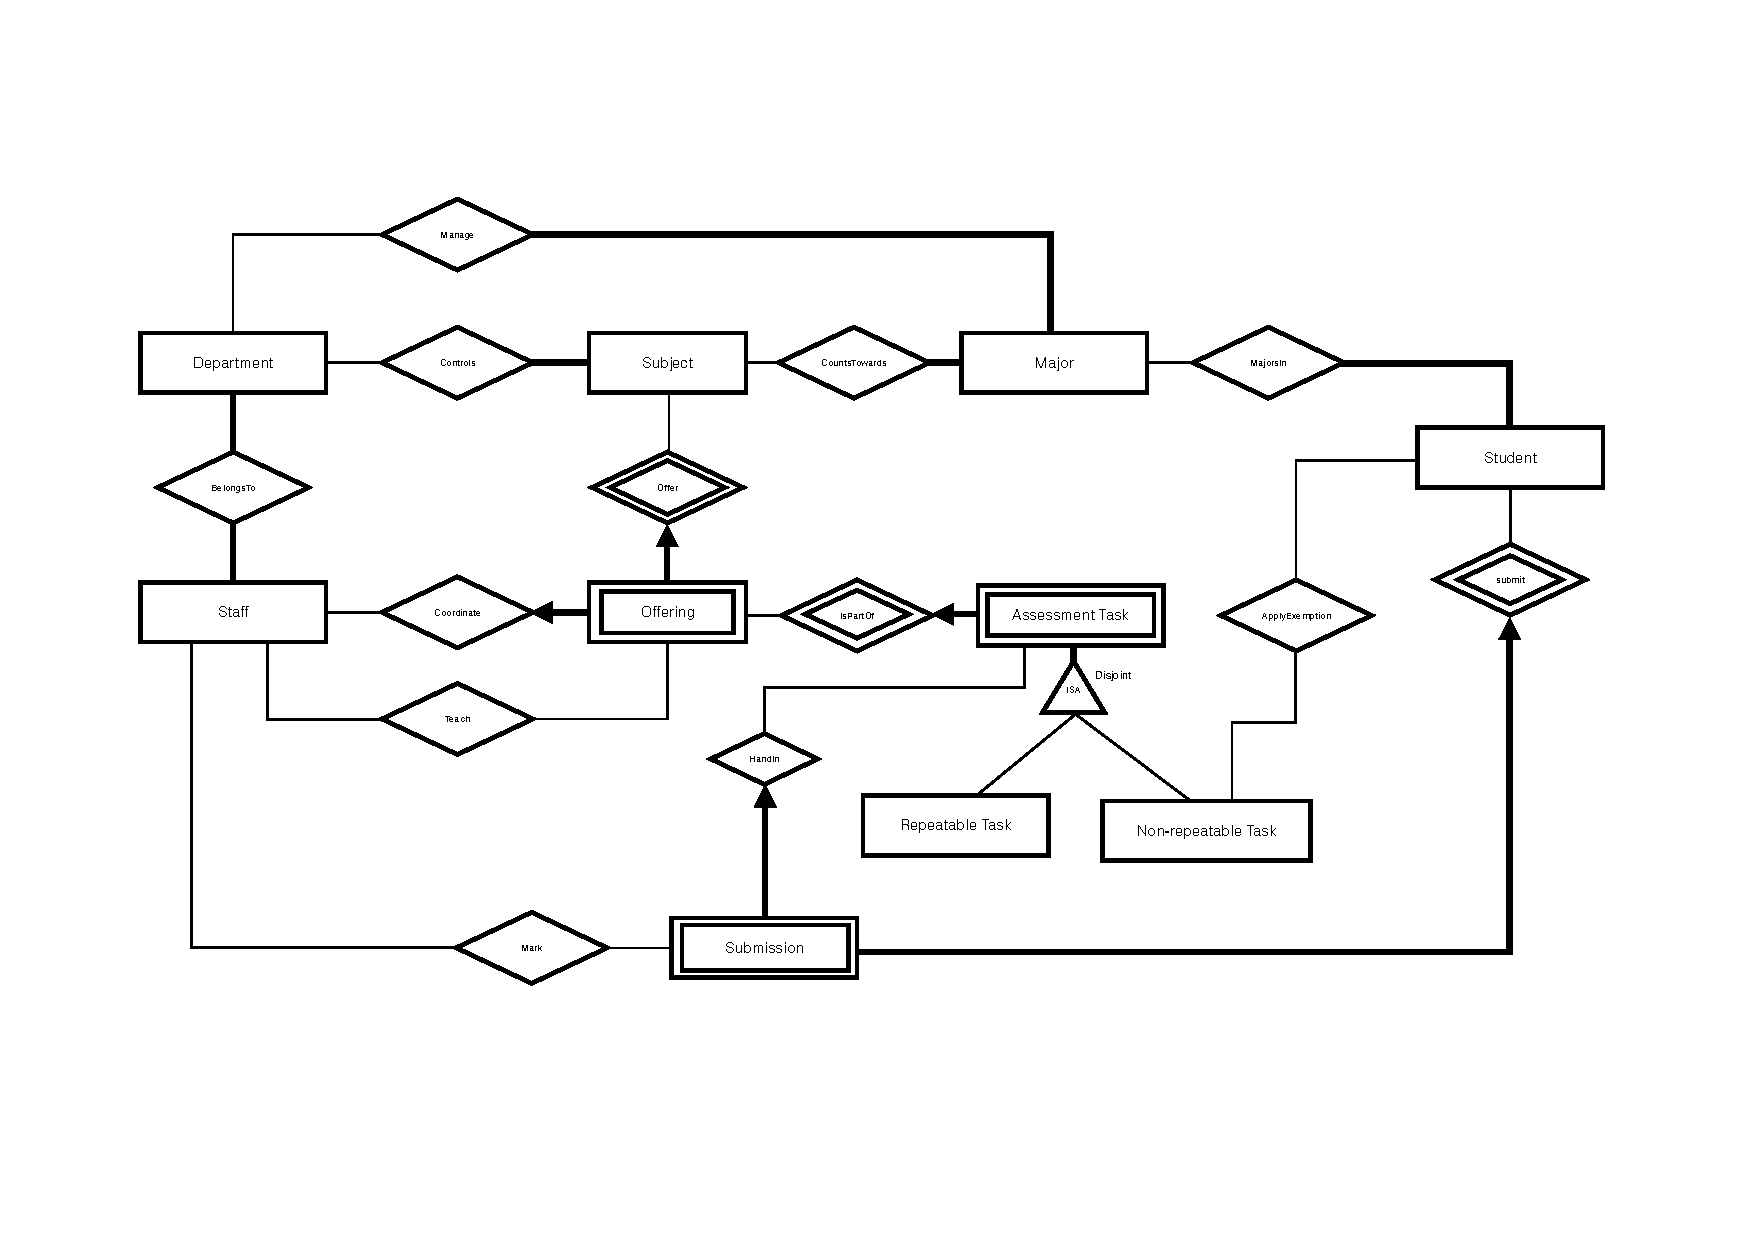
\includepdf[pages={1-6}]{graphs/ER-diagram.pdf}

\section*{Part B}


\subsection*{Decision}

\subsubsection*{1. \texttt{Offering} as a Weak Entity Set}
In the ER diagram, we modeled \texttt{Offering} as a weak entity. The reason is that simply recording the \texttt{semester} and \texttt{year} is not enough to uniquely identify which course the offering corresponds to, making it impossible to determine the associated course.
\begin{itemize}
    \item To address this issue, we modeled \texttt{Offering} as a weak entity with \texttt{semester} and \texttt{year} as discriminators. By combining this with the primary key of \texttt{Subject}, we can uniquely identify a course offering. This decision ensures that each offering is correctly linked to its respective course while retaining all relevant information.
\end{itemize}

\subsubsection*{2. Convert "submit" from a relationship into a new entity set}

We modeled "submit" as an entity set called \texttt{Submission} rather than a relationship because "submit" involves connections with \texttt{Assessment, Student, and Staff}, and it has its own attributes: \texttt{mark, date, and time}. Modeling it as an entity better captures the relationships between these entity sets in a more intuitive way compared to modeling it as a relationship.

\subsubsection*{3. \texttt{Submission} as a Weak Entity Set}
Since the spec does not specify the primary key for \texttt{Submission}, and the attributes of \texttt{Submission} alone cannot uniquely distinguish it, we decided to use the submission \texttt{time, date}, and the student's \texttt{StudentKey} as a composite primary key. \texttt{Submission} is modeled as a weak entity set, with the date and time as its discriminators. This decision is based on the fact that a student cannot submit two submissions at the exact same time.

\subsubsection*{4. ISA hierarchy for Assessment Task}

For the Assessment Task, we encountered a design challenge due to the differing mechanisms between repeatable and non-repeatable tasks. If we were to represent all tasks using a single \texttt{Assessment Task} entity, both types of tasks would need to store their unique attributes in the same table, and since different types of \texttt{Assessment Task} have different relationships with other entities, this could complicate the design of the relational schema. To address this issue, we decided to use an ISA hierarchy to represent repeatable and non-repeatable tasks separately.

\subsubsection*{5. \texttt{Exemption As Relationship}}

In the early stages of the design, we realized that we had not captured the relationship between Exemption and students. We came up with two ideas. 
    \begin{itemize}
        \item The first was to model Exemption as a weak entity of Student, with "date" as the discriminator. However, this was insufficient to distinguish exemptions, as there could be a case where a student applies for two exemptions for non-repeatable tasks on the same day.

        \item The second approach was to model \texttt{Exemption} as a many-to-many relationship, with \texttt{date, text, and status} as attributes of the relationship. While this approach addressed the limitations of the first method, it introduced another issue: in the current scenario, a student can only submit one exemption request for the same non-repeatable assessment.
    \end{itemize}
In comparison, we chose to model \texttt{exemption} as a relationship.

\subsubsection*{6. \texttt{Assessment} as a Weak Entity Set}

For the \texttt{Assessment Task}, the description does not specify which attribute should be used for PK. Considering that each assessment task corresponds to a specific offering, and typically (in a university setting), no two assessment tasks under the same offering will have the same name, we decided to model the \texttt{Assessment Task} as a weak entity set, with \texttt{Name} as the discriminator. Its corresponding strong entity set is \texttt{Offering}.

\subsection*{Clarifications and Assumption}

\subsubsection*{1. \texttt{Subject}'s PK}
Since the specification does not mention how subjects are identified, based on real-world scenarios where different subjects typically have different names, we chose \texttt{Name} as the primary key.

\subsubsection*{2. \texttt{Staff-Department} Relationship}
The specification does not explicitly state whether a staff member can belong to multiple departments or if they must belong to exactly one department, and whether a staff member must belong to a department or if they can exist without any department. In this case, we assumed that each staff member must belong to \textbf{at least one department}, and they can belong to \textbf{multiple} apartments. This assumption reflects the real-world scenario where staff members are typically part of an organizational structure and report to a department.

\subsubsection*{3. \texttt{Staff-Submission} Relationship}
The specification does not clarify whether a submission can be marked by multiple staff members or only by one. We have assumed that a submission can be marked by \textbf{multiple} staff members, and therefore, we modeled this as a \textbf{many-to-many} relationship between submissions and staff. In real-world scenarios, it is common for certain assessments, especially large-scale or critical tasks, to be reviewed or graded by multiple staff members to ensure fairness.

\subsubsection*{4. \texttt{Student-Major} Relationship}

The specification does not explicitly state whether a student can belong to only one major. Based on real-world scenarios and ED post \texttt{\#459}, we assumed that a student can belong to one or more majors. The relationship from student to major is many-to-one, with student having full participation.

\subsubsection*{5. \texttt{Major}'s PK}
We assume that the primary key (PK) for a \texttt{Major} is its \texttt{Name}, based on real-world conventions.



\subsection*{Strength}
\begin{enumerate}
    \item One key strength of our ER diagram is the use of the \textbf{ISA} structure to model the relationship between \texttt{Assessment Task, Non-repeatable Assessment, and Repeatable Assessment}. This design decision preventing unnecessary redundancy in the database and store information efficiently. For example, only \texttt{Non-Repeatable} Assessments can have additional relationship \texttt{ApplyExemption}. This includes tracking the text of the request, the date it was made, and whether or not the request was approved.

    \item Modeling \texttt{Offering} as a weak entity set effectively captures the "course offering" as described in the spec. We can avoid adding a new primary key by distinguishing different offerings using the primary key of \texttt{Subject} along with the \texttt{year} and \texttt{semester} of the \texttt{Offering}. This design clarifies the relationship between Subject and Offering, while avoiding unnecessary attributes.
\end{enumerate}

\subsection*{Limitation}
\begin{enumerate}
    \item In the current design, exemption is modeled as a many-to-many relationship: \texttt{ApplyExemption}. However, there is an issue with this design: a student can only submit one exemption request for the same non-repeatable assessment. In reality, a student may submit multiple requests for the same assessment, such as when previous exemption requests were denied, and only the final one was approved.

    \item According to the spec, a student can only submit once for the same non-repeatable assessment. However, this restriction is not reflected in the diagram. In the current design, students can submit multiple times. To enforce this restriction, we need to ensure that a submission is unique for a student and a non-repeatable assessment, which is not achievable in the current diagram.

    \item The system needs to record the grading policy for assessment tasks that allow multiple submissions. For example, only the last submission might be graded, the highest score might be taken, or points may be deducted based on the number of submissions. These complex grading rules and policies are difficult to capture in a standard ER diagram and typically need to be implemented through business logic in the application, rather than solely through the database structure.
\end{enumerate}
\end{document}
